\chapter{Аналитическая часть}

В этой части рассматриваются анализ предметной области, известных решений и моделей баз данных, формализации задачи и ролей.

\section{Анализ предметной области}

Организация мероприятий -- это многогранный и трудоемкий процесс, который требует внимания к деталям и учета множества факторов. От выбора подходящей локации до составления списка гостей, от планирования бюджета до подготовки меню -- каждый этап организации требует тщательной проработки. В ходе подготовки организаторы сталкиваются с рядом типичных вопросов, таких как: «Что необходимо приобрести для мероприятия?», «Какое количество гостей ожидается?» и «Какова стоимость участия?». Эти вопросы, хотя и кажутся простыми, но требуют значительных временных и организационных затрат, особенно если мероприятие масштабное или включает множество участников~\cite{lit1}.

Для упрощения этого процесса были разработаны специализированные инструменты -- планировщики мероприятий. Эти приложения предназначены для того, чтобы объединить все этапы организации мероприятия в единую систему, сделать процесс планирования более структурированным и прозрачным. Планировщик мероприятий позволяет организаторам:
\begin{enumerate}
	\item систематизировать задачи -- разбить процесс организации на этапы и подзадачи;
	\item координировать участников -- вести список гостей, учитывать их предпочтения и информировать о деталях мероприятия;
	\item управлять бюджетом -- учитывать расходы и планировать финансы, чтобы избежать непредвиденных затрат;
	\item контролировать сроки -- устанавливать дедлайны для каждой задачи и отслеживать их выполнение.
\end{enumerate}


\section{Анализ известных решений}

Организация мероприятий всегда была важной и востребованной сферой, потому для упрощения этого процесса были разработаны специализированные информационные системы, которые автоматизируют множество задач. Наиболее популярными являются:
\begin{enumerate}
	\item Eventbrite -- платформа для организации мероприятий, которая позволяет создавать страницы событий, продавать билеты онлайн, собирать данные о посетителях и управлять регистрациями~\cite{lit2};
	\item Cvent -- профессиональная платформа для организации мероприятий, которая предлагает комплексные решения для планирования, управления гостями, бюджетирования и аналитики~\cite{lit3};
	\item Trello -- инструмент для управления проектами и задачами, который можно адаптировать для планирования мероприятий~\cite{lit4}.
\end{enumerate}

Критерии сравнения известных решений и результаты их сравнительного анализа представлены в таблицах~\ref{tbl:criteria} и~\ref{tbl:results} соответственно.

\begin{table}[h]
	\centering
	\caption{Критерии сравнения известных решений}
	\begin{tabularx}{\textwidth}{|X|X|}
		\hline
		\textbf{Критерий} & \textbf{Описание} \\
		\hline
		Аккаунт & Возможность иметь аккаунт \\
		\hline
		Бесплатный доступ & Бесплатный доступ ко всем возможностям приложения \\
		\hline
		Привилегии участников & Возможность выдавать участникам роли с привилегиями \\
		\hline
		Рейтинг & Формирование оценки мероприятия по оставленным отзывам \\
		\hline
	\end{tabularx}
	\label{tbl:criteria}
\end{table}

\begin{table}[h]
	\centering
	\caption{Результаты сравнительного анализа известных решений}
	\begin{tabularx}{\textwidth}{|X|X|X|X|}
		\hline
		\textbf{Критерий} & \textbf{Eventbrite} & \textbf{Cvent} & \textbf{Trello} \\
		\hline
		Аккаунт & + & + & + \\
		\hline
		Бесплатный доступ & - & - & + \\
		\hline
		Привилегии участников & - & + & - \\
		\hline
		Рейтинг & + & + & - \\
		\hline
	\end{tabularx}
	\label{tbl:results}
\end{table}

Ни одно из рассматриваемых решений не обеспечивает пользователя всеми необходимыми функциями для организации мероприятий.

\section{Формализация задачи}

Необходимо спроектировать и реализовать базу данных, которая будет хранить данные о пользователях, мероприятиях и отзывах. Также требуется разработать приложение с функционалом для просмотра, добавления, редактирования и удаления информации.

\section{Формализация данных}

Исходя из анализа предметной области, можно выделить следующие ключевые группы данных:
\begin{itemize}[label=--]
	\item локация;
	\item мероприятие;
	\item день мероприятия;
	\item участник мероприятия;
	\item меню мероприятия;
	\item предмет меню;
	\item отзыв;
	\item пользователь.
\end{itemize}

Группы данных и сведения о них представлены в таблице~\ref{tbl:data-groups}

\begin{table}[h]
	\centering
	\caption{Группы данных и их сведения}
	\begin{tabularx}{\textwidth}{|X|X|}
		\hline
		\textbf{Группа данных} & \textbf{Сведения} \\
		\hline
		Локация & Название, описание, цена аренды, вместимость \\
		\hline
		Мероприятие & Название, описание, дата, количество участников, количество дней, локация, рейтинг \\
		\hline
		День мероприятия & Название, порядковый номер, описание, цена посещения, меню \\
		\hline
		Отзыв & Комментарий, рейтинг, участник мероприятия \\
		\hline
		Пользователь & Имя, телефон, гендер, роль, права доступа, пароль \\
		\hline
		Участник мероприятия & Имя, тип, факт оплаты \\
		\hline
		Меню мероприятия & Название, стоимость \\
		\hline
		Предмет меню & Название, тип, цена \\
		\hline
	\end{tabularx}
	\label{tbl:data-groups}
\end{table}

ER-диаграмма сущностей в нотации Чена представлена на рисунке~\ref{fig:er-diagram}.

\begin{figure}[h]
	\centering
	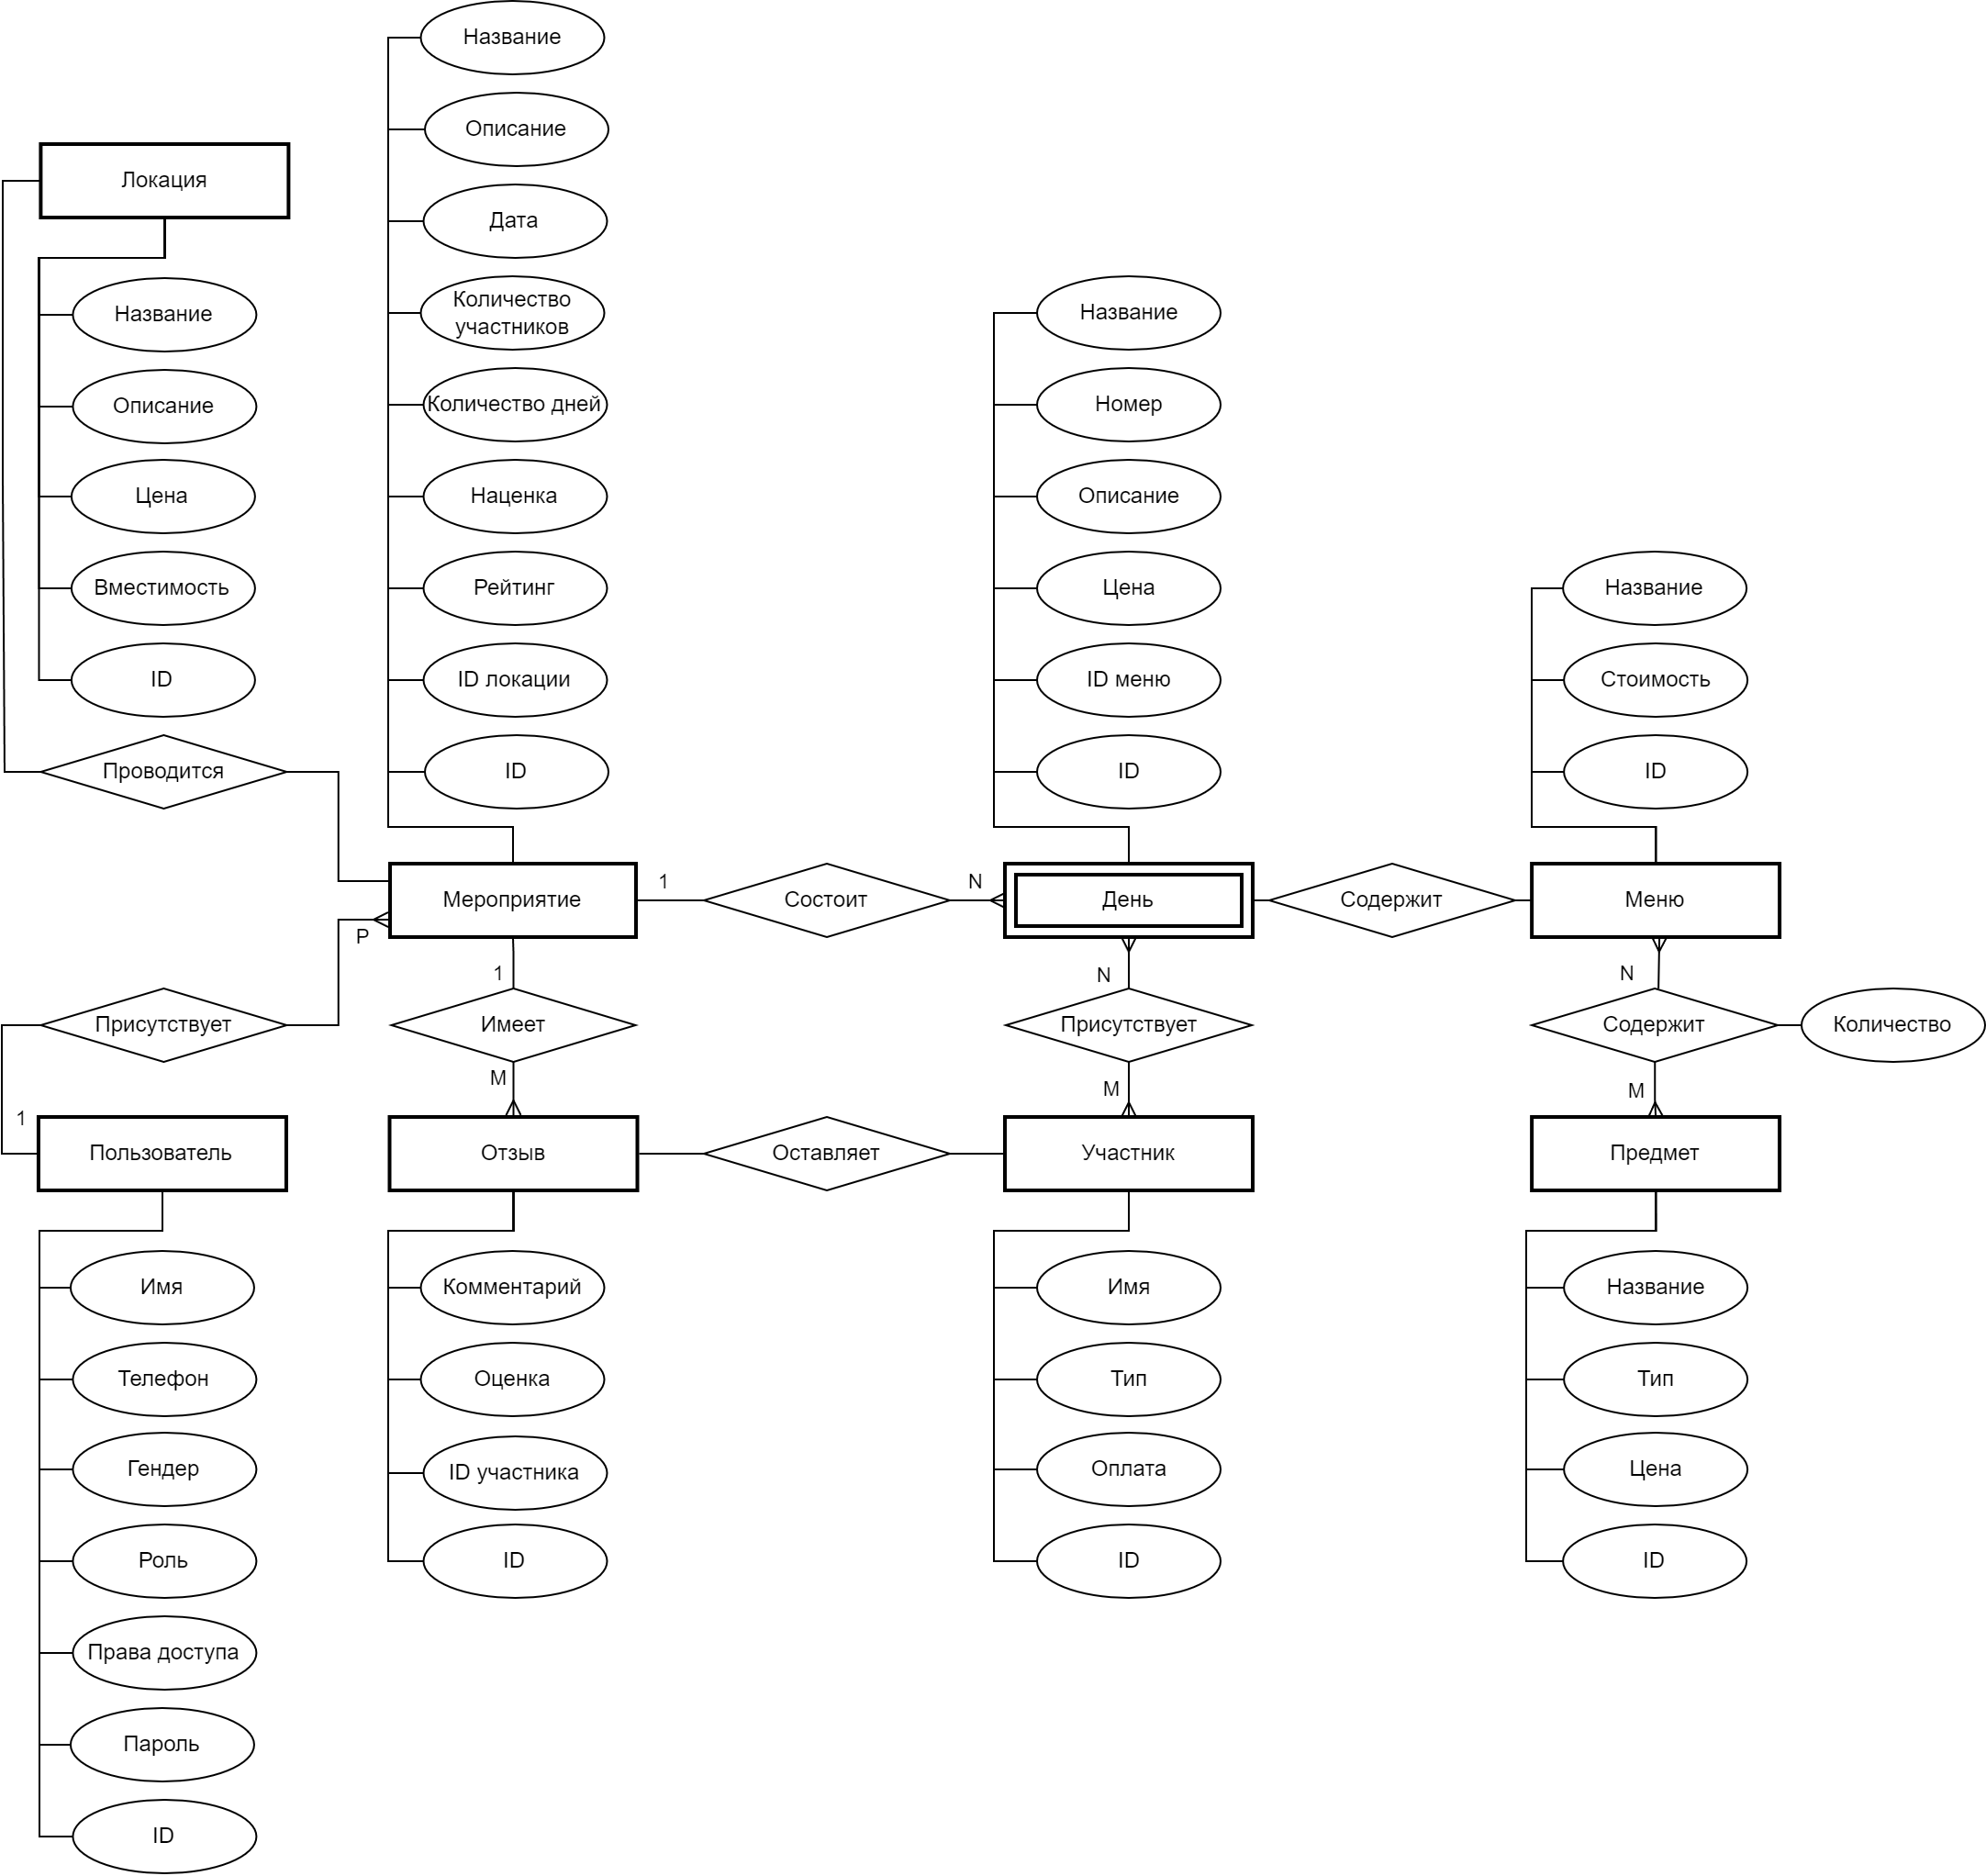
\includegraphics[width=1\textwidth]{images/er-diagram.png}
	\caption{ER-диаграмма сущностей в нотации Чена} 
	\label{fig:er-diagram} 
\end{figure}

\section{Формализация ролей}

В разрабатываемой системе выделяются три категории пользователей:
\begin{enumerate}
	\item гость -- неавторизованный пользователь, который может регистрироваться, входить в систему и просматривать информацию о мероприятиях;
	\item зарегистрированный пользователь -- может просматривать данные о мероприятиях, подавать и удалять заявки на участие, а также оставлять и удалять отзывы;
	\item администратор -- обладает правами на просмотр, добавление и изменение данных о мероприятиях, пользователях и отзывах.
\end{enumerate}

Множества значений перечисляемых сведений представлены в таблице~\ref{tbl:data-groups-types}.

\begin{table}[h]
	\centering
	\caption{Множества значений перечисляемых сведений}
	\begin{tabularx}{\textwidth}{|X|X|X|}
		\hline
		\textbf{Группа данных} & \textbf{Сведение} & \textbf{Множество значений} \\
		\hline
		Пользователь & Роль & Гость, зарегистрированный пользователь, администратор \\
		\cline{2-3}
		 & Гендер & Мужской, женский \\
		\hline
		Участник мероприятия & Тип & Простой участник, VIP, организатор \\
		\hline
		Предмет меню & Тип & Однодневный, многодневный \\
		\hline
	\end{tabularx}
	\label{tbl:data-groups-types}
\end{table}



\section{Анализ моделей баз данных}

\section{Вывод}

В аналитической части работы был проведен анализ...

\clearpage
